\documentclass[tekniskrapport/tech.tex]{subfiles}

\begin{document}

\section{Kommunikationsmodul}
Kommunikationsmodulen styr bilen och kommunicerar med fjärrklienten.
Sensorvärden från sensormodulen tolkas av kommunikationsmodulen som därefter
skickar felvärden till styrmodulen.

Bildbehandling utförs av kommunikationsmodulen för att
avgöra bilens position i vägfilen och upptäcka stopplinjer. Med hjälp av
kamerans bilder på vägen skapas ett felvärde som kan användas för att justera
taxins riktning.

Kommunikation med fjärrklienten sköts av kommunikationsmodulen för
att skicka sensorvärden och annan relevant information. Modulen tar
även emot uppdrag.

Autonomitet utförs av kommunikationsmodulen för att utföra uppdraget.
Kommunikationsmodulen hämtar sensordata från sensormodulen och bildbehandlar
kamerabilderna för att utföra beslut i realtid. Besluten skickas i form av fel-
och styrvärden till styrmodulen.

Kommunikationsmodulens program är skriven i både C och C++. Bildbehandlingen är
skriven i C++ medan resten av programmet är implementerad med C. De olika
delarna kompileras separat och länkas sedan ihop med kompilatorn för C++.
Programmet består av tre trådar; en huvudtråd som hanterar uppdrag och
bildbehandlar, samt en tråd som sköter kommunikation via SPI och en som svarar
på kommandon från fjärrklienten via TCP/IP. SPI:n och servern sköts i separata
trådar eftersom de väntar mycket och blockerar den nuvarande tråden.


\subsection{Hårdvaruimplementation} 
Kommunikationsmodulen har implementerats i en Raspberry Pi 3B. Raspberry Pi 3B,
har en fyrkärnig processor med en hastighet på 1.2 GHz vilket har kunnat
utnyttjas inte minst vid bildbehandlingen. Med 40-pinnar som kan utnyttjas som
spänningskällor, jord, programmerbara GPIO-portar samt seriella bussar, har
detta utnyttjats för att med SPI-protokollet använda Raspberry Pi:n som master
för två slavar. Då kommunikationen med en fjärrklient sker via WiFi har det
inbyggda 802.11n trådlösa LAN:et varit fullt kapabelt. Det trådlösa
nätverkskortet hade med en bra implementation även kunnat strömma video. Mitt
på Pi:en hittar man en CSI-port som används för att ansluta Raspberry Pi
kompatibla kameror. Kameran som används på kommunikations modulen är en
Raspberry Pi kamera med påsatt vidvinkelobjektiv som kan se i en 160 graders vy.
Kameran har även stöd för två infrarödastrålkastare, men detta används inte då
mörkerseende inte är något som prioriterats. Spänningskällor finns i både 3V3
och 5V.

\subsection{Programstruktur}
Programmet på kommandomodulen består av följande filer

\begin{labeling}{wwwwwwwwww}
    \item[server.c] Server som anropar kommandofunktioner vid förfrågan från
        klient från separat tråd.
	\item[spi.c] Lågnivåfunktioner för SPI.
    \item[bus.c] Hantering av SPI-buss, utför kommandon på bussen och anropar
        signalhanterare från separat tråd.
    \item[ip/img\_proc.cpp] Bildbehandling med OpenCV.
    \item[objective.c] Utförarande av uppdrag.
    \item[main.c] Huvudloop och implementation av signalhanterare för buss och
        server.
\end{labeling}

\paragraph{Huvudtråden} startar servern och busshanteraren. Därefter startar
den huvudloopen som antingen tar styrvärden utifrån användarens kommandon via
servern eller från uppdragshanteraren med hjälp av bildbehandling av den
senaste bilden från kameran. Därefter schemaläggs skrivning av de nya
styrvärdena till styrmodulen. Dessutom schemaläggs hämtning av sensorvärden
från sensorerna.

\paragraph{Servern} erhåller en sockel för nya anslutningar och en för att
skicka och ta emot meddelanden för en aktiv anslutning. Servern kan därmed
endast erhålla en anslutning i taget. Anslutningssockeln är bunden till en port
mellan 9000 och 9100. När en anslutning förfrågas eller om ett meddelande tas
emot väcks servern och accepterar eller tar emot meddelande. Om en
anslutningsförfrågan tas emot skapas en ny sockel för meddelanden och
överskrider den tidigare sockeln om den finns. Om ett meddelande med ett
giltigt kommando tas emot anropas kommandots funktion som utför sin handling
och genererar ett svarsmeddelande som servern sedan vidarebefogar till
klienten. Därefter sover servern igen tills en ny förfrågan tas emot.

\paragraph{Busshanteraren} fungerar på liknande sätt som servern. Den sover
tills en förfrågan sker. Förfrågningarna kommer däremot från andra trådar i
programmet istället för klienten. Om flera förfrågningar sker innan servern har
utfört den nuvarande kommer de nya meddelandena köas i sockeln av
operativsystemet. Det finns dock ingen sockel att köa förfrågningar i för
busshanteraren. Därför har en länkad lista implementerats för att kunna erhålla
flera förfrågningar. När en förfrågan sker läggs den sist i kön och
busshanteraren väcks om den sover. Om kön redan innehåller en förfrågan med
samma kommandotyp ersätts den med den nya förfrågan. Busshanteraren utför
därefter förfrågan via SPI och om kommandot gick igenom anropas
signalhanteraren för det kommandot. Om kommandot inte gick igenom läggs
kommandot sist i kön om ett nyare förfrågan av samma typ inte redan finns i
kön. Annars kastas den äldre förfrågan bort.

\subsection{Bildbehandling}
Bildbehandlings processen sker genom ett program skrivet i C++.

\subsubsection{Upptäckt av linjer}
Upptäckandet av linjer/kanter på banan sker genom hanteringen av varje
bild/frame som programmet tar emot från kameran. Varje bild går igenom en
process som börjar med att förberedda bilden genom att filtrera den för att
först underlätta kanters upptäckande och sedan linjerna inom ett bestämt område
av intresse (Region of Interest ROI).

Processen börjar med att filtrera bilden med den så kallade Gauss filter där
bilden faltas med en Gauss kernel med tanke på att filtrera bort brus. Den
filtrerade bilden omvandlas sedan till en monokromatisk bild vilket underlättar
bildbehandlingen och som är möjligt tack vare att bildbehandlingsprogrammet
inte använder sig utav specifika färger för att upptäcka linjer på vägen utan
det arbetar med de linjerna inom ROI och klassar dem enligt deras lutning och
position. Det här innebär att upptäckandet av linjer ska vara möjligt utfört
oberoende på vilka färger vägen kunde ha. 

Det sista steget innan kanterna upptäcks är att segmentera bilden genom att
från openCV använda threshold funktionen som erbjuder olika typer av threshold
operationer vilka möjliggör att skilja mellan olika region/objekt som önskas
analysera baserad på hur intensiteten hos varje pixel varierar mellan objektet
och bakgrunden. Programmet använder sig av Otsu threshold metod vilken själv
räknar ut en threshold värdet som bäst passar bilden. Den använda threshold
funktionen returnera den nya bilden vilken visas på bilden...

Nu när bilden är förbered för kanters upptäckande används funktionen Canny
(från openCv), som applicerar Canny algoritmen vilken identifierar alla kanter
som finns i bilden. Resultatet visas på bilden ... 

Som tidigare nämnts, upptäcks linjerna inom ROI. ROI bestäms baserad på hur
mycket av bilden vill användas för att hitta linjer; hur mycket som är
tillräckligt för tolkningen och senare hanteringen av alla linjer som hittas på
vägen. ROI är en polygon av 6 punkter som enkelt kan anpassas vid behov och som
visas på bilden ...   

Efter att bilden är hel filtrerad och ROI bestämd, används Hough transformen
för att hitta linjer enligt bestämda parametrar som varje linje ska uppfylla i
transformen för att bli klassa som linje. OpenCV erbjuder två typer av
funktioner som applicerar transformen och programmet använder sig av den
probabilistiska metoden vilken ökar beräknings hastighet utan att minska
precisionen. Efter användningen av Hough transformen kan programmet tolka de
upptäckade linjerna.

\subsubsection{Tolkning av linjer}
Det första som görs med alla linjer som hittas på bilden är att klassificera de
som vänsterlinje, högerlinje, stopplinje eller annan linje. Dessa färgas gröna,
blå, röda och gråa respektive. Därefter beräknas x-positionen av filens
högerkant vid ett $y=l_y$ genom att räkna ut medianvärdet av x-positionerna där
alla högerlinjer korsar $y=l_y$. På samma sätt räknas vänsterkantens position i
x-led ut. Därifrån kan filens bredd $w$ och mittpunkten $l_x$ räknas ut vid
$y=l_y$. Felvärdet beräknas därefter genom att jämföra $l_x$ med bildens
mittpunkten.

\begin{wrapfigure}{r}{0.3\linewidth}
    \begin{center}
        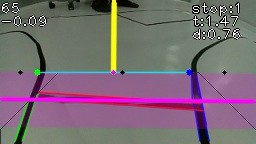
\includegraphics[width=\linewidth]{tekniskrapport/figures/opencv.jpg}
    \end{center}
    \caption{Klassificering och tolkning av linjer från kamera.}
\end{wrapfigure}

Vänster och högerlinjerna används dessutom för att uppskatta filens riktning.
Detta görs genom att addera alla sidolinjer som vektorer och därmed få en
vinkelsumma $\vec{v}$ (gul färg) som har en genomsnittlig riktning. En linje
$D$ som korsar $\vec{l}=(l_x, l_y)$ och har riktningsvektorn $\vec{v}$ används
för att klassificera nästa bilds linjer. Linjer som korsar $D$ och har en stor
vinkel till $D$ klassificeras som stopplinjer. Linjer vars båda punkter
befinner sig till höger om $D$ och inte har en särskilt stor vinkel till $D$
klassificeras som en högerlinje. På samma sätt klassificeras vänsterlinjer.

Om antingen vänster eller höger kant inte skulle upptäckas används den
uppskattade bredden för att räkna ut var mittpunkten av filen är.

Linjer som klassificeras som stopplinjer används för att bestämma om en
stopplinje har korsats. Stopplinjens position i y-led uppskattas utifrån den
tidigare bilden. Endast linjer som är inom ett visst avstånd till den
uppskattade positition antas vara del av stopplinjen. Till en början antas den
vara högst upp i ROI:n. När stopplinjen har upptäckts hela vägen från toppen av
ROI:n till botten av bilden utan att gå för långt ifrån uppskattningen
registreras en passering av stopplinjen. Om linjen inte skulle upptäckas under
en bild flyttas uppskattningen tillbaka till toppen av ROI:n.
  
\subsection{Uppdrag} \label{sec:comm-mission}
Uppdragshanteraren körs i huvudloopen. Det första uppdragshanteraren gör för
varje iteration är att kolla om ett nuvarande kommando är aktivt. Annars hämtar
den ett nytt från kommandokön. Om kön är tom är uppdraget avslutat. Om kön
istället har ett nuvarande kommando utförs bildbehandling och styrvärdena sätts
till normalhastighet och styrfelvärde från bildbehandlingen. 

\begin{labeling}{wwww}
    \item[\commIgnore] Kör förbi stopplinjen utan att stanna.
    \item[\commStop] Stanna framför stopplinjen, fortsätt efter några sekunder
    om kön inte är tom.
    \item[\commPark] Parkera i fickan till höger efter stopplinjen, lämna
    parkeringen och fortsätt efter några sekunder om kön inte är tom.
    \item[\commEnter] Sväng höger in i rondellen och hitta rondellens körfil.
    \item[\commContinue] Kör förbi stopplinje och håll till vänster.
    \item[\commExit] Sväng höger ut ur rondellen och hitta körfilen.
\end{labeling}

\end{document}
